% -*- TeX-command-extra-options: "-shell-escape"; TeX-engine: luatex; -*-
\documentclass[a4paper, parskip]{scrartcl}

\usepackage{graphicx}
\usepackage{enumitem}
\usepackage[ngerman]{babel}
\usepackage{fontspec}
\usepackage{cprotect}
\usepackage{subfig}
\usepackage{graphicx}
\usepackage{hyperref}
\usepackage{wasysym}
\usepackage{tikz}
\usepackage{tikz-qtree}
\usepackage{minted}
\usepackage[backend=biber]{biblatex}
\usepackage{xcolor}
\usepackage{caption}

\newenvironment{code}{\captionsetup{type=listing}}{}

\hypersetup{
    colorlinks,
    linkcolor={red!50!black},
    citecolor={blue!50!black},
    urlcolor={blue!80!black}
}

\addbibresource{main.bib}

\usetikzlibrary{arrows,shapes,shapes.multipart,calc,chains,positioning,fit,matrix,datavisualization}
\tikzset{
  every tree node/.style = {align=center, inner sep=5pt, text centered, font=\sffamily, rectangle, black, draw=black, very thick},
  every leaf node/.style = {draw=none},
  n/.style = {draw=none},
  level distance=1.5cm,sibling distance=0.5cm
}

\title{Verifizierte Implementierung einer Mapping-Datenbank in Coq}
\author{Benno Fünfstück}
\date{\today}
\pagestyle{empty}

\begin{document}

\begin{raggedright}

\sectfont\Large
Martin-Andersen-Nexö-Gymnasium Dresden
\vspace{1.5 cm}


\noindent
Dokumentation zur wissenenschaftlichen Projektarbeit
\vspace{1.5 cm}

\large
\noindent
\begin{tabbing}
Thema: \=\mdseries Verifizierte Implementierung einer\\
\>\mdseries Mapping-Datenbank in Coq
\end{tabbing}
\vspace{3 cm}

\noindent
\begin{tabbing}
vorgelegt von: \=\mdseries Benno Fünfstück
\end{tabbing}
\vspace{3 cm}

\noindent
\begin{tabbing}
externer Betreuer: \=\mdseries Dr. Hendrik Tews\\
                   \>\mdseries Dr. Thomas Türk\\
                   \\
                   \>\mdseries FireEye Technologie Deutschland GmbH                    
\end{tabbing}
\vspace{1.0 cm}

\noindent
\begin{tabbing}
schulischer Betreuer:
\end{tabbing}
\vspace{1.0 cm}
Dresden, 15.06.2015

\end{raggedright}
\cleardoublepage


\subsection*{Kurzfassung}
Aktuell verbreitete Betriebssystemkerne sind zu komplex, um sie vollständig zu testen.
Doch gerade Fehler im Systemkern stellen ein großes Sicherheitsrisiko dar, da sie die Umgehung der meisten anderen Sicherheitsmaßnahmen ermöglichen. 
Microkerne versuchen deshalb, möglichst viele Funktionen außerhalb des Kerns zu implementieren und damit die Komplexität des sicherheitskritischen Teils zu minimieren.

Selbst dann können jedoch nicht alle möglichen Fälle getestet werden.
In dieser Arbeit wird deshalb Coq zur formalen Verifikation eingesetzt.
Es wird eine verifizierte Implementierung von AVL-Bäumen entwickelt, die als finite Maps viele Anwendungsmöglichkeiten besitzen.
Durch die Verifikation wurden mehrere Fehler in der Implementierung gefunden, doch die Beweise garantieren, dass keine weiteren Fehler existieren.

Darauf aufbauend wird ein Modell einer Mapping-Datenbank entwickelt, wobei wichtige Eigenschaften bewiesen werden.
So wird die Korrektheit dieser zentralen Komponente sichergestellt, die der Verwaltung der Rechte von Prozessen eines Microkern-basierten Systems dient.
\bigskip\bigskip


\subsection*{Abstract}
Commonly used system kernels are too complex to be fully tested.
However, bugs in the kernel are a high security risk, since they can lead to the circumvention of most other security measures.
Microkernels therefore try to implement as many functions as possible outside of the kernel, thereby reducing the complexitiy of the security-critical part.

Even then, not all cases can be tested.
To remedy this, the work uses Coq in order to perform formal verification.
I develop a verified implementation of AVL trees, which have many applications as finite maps.
Through the verification, multiple bugs were found in the implementation.
The proofs guarantee that no further bugs exist.

The formalization of AVL trees is used to develop a mapping database and prove important properties.
Those properties imply the correctness of this central component, which manages the rights of processes in a microkernel-based system.
\cleardoublepage

\pagestyle{plain}
\setcounter{page}{1}
\tableofcontents{}
\newpage

\section{Einleitung}
Mit immer weiter steigender Rechenleistung von Computern nimmt auch die Komplexität der Software zu. 
So enthält der Linux-Kern\footnote{Version 3.18} mittlerweile fast 19 Millionen Zeilen Quellcode.\autocite{linux-dev}
Andere aktuelle Betriebssysteme wie Microsoft Windows 7 oder Mac OSX 10.4 besitzen ähnlich viele Quellcodezeilen, wenn nicht sogar mehr.\autocite{common-loc}

Bei dieser Komplexität ist es unmöglich, die Fehlerfreiheit sicherzustellen.
Im Linuxkern werden immer wieder neue Fehler und Sicherheitslücken aufgedeckt.
Schätzungen zufolge existieren in Software etwa 3 Fehler pro 1000 Zeilen, wovon rund 10\% sicherheitskritisch sind.
In 19 Millionen Zeilen existieren nach dieser Rechnung somit rund 5500 sicherheitskritische Fehler.

Doch gerade Systemkerne stellen einen besonders sicherheitsrelevanten Teil eines Betriebssystems dar.
Da sie im privilegierten Modus laufen, welcher direkten Hardwarezugriff erlaubt, kann ein Fehler im Kern dazu führen, dass auch Schadcode im privilegierten Modus ausgeführt wird.
Im privilegierten Modus kann der Schadcode alle anderen Sicherheitsmechanismen umgehen, weil er die volle Kontrolle über das System hat.

Microkerne haben deshalb das Ziel, den im Kern und damit den im privilegierten Modus laufenden Teil zu minimieren. 
Es werden so viele Funktionen wie möglich außerhalb des Kerns im unprivilegierten Modus implementiert. 
Außerdem können die einzelnen Komponenten, die aus dem Kern ausgelagert wurden, nun durch die vom Kern bereitgestellten Isolationsfunktionen voneinander getrennt werden. 
Das hat mehrere Vorteile.
Zum einen ist die Komplexität der einzelnen Komponenten nun geringer, da sie durch die zusätzliche Isolation nicht mehr so stark von den anderen Komponenten abhängen. 
Damit können sie einfacher auf Korrektheit überprüft werden und enthalten so weniger Fehler. 
Da sie voneinander isoliert sind, wirkt sich ein Fehler in einer Komponente nicht auf andere Komponenten aus.
Zum anderen ist das System jetzt auch flexibler, denn die einzelnen Komponenten können zur Laufzeit des Systems ohne Neustart des Kerns ausgetauscht werden.

Der minimalistische Ansatz von Microkernen führt dazu, dass auch für die Verwaltung der Rechte von Prozessen nur die Mechanismen, um Prozessen Rechte zu geben oder zu entziehen, im Kern selbst implementiert werden.
Die Festlegung von Richtlinien und die Verwaltung der Rechte der Prozesse wird außerhalb des Kerns implementiert.
Dazu wird eine Mapping-Datenbank benötigt, die die aktuellen Rechte der einzelnen Prozesse speichert.

Um Fehler zu vermeiden, muss die Mapping-Datenbank auf ihre Korrektheit überprüft werden.
Eine Möglichkeit dazu stellt das Testen der Mapping-Datenbank in verschiedenen Szenarien dar.
Allerdings ist es selbst mit automatisierten Methoden unmöglich, dabei alle Fälle abzudecken.
In dieser Arbeit werden deshalb formale Methoden eingesetzt, um die Korrektheit mit mathematischen Methoden zu beweisen.
Im Gegensatz zum einfachen Testen, wobei die Implementierung für mehrere Beispielsituationen überprüft wird, kann eine Eigenschaft der Implementierung mithilfe der formalen Verifikation für alle Eingaben bewiesen werden.

In dieser Arbeit geht es um die Entwicklung einer in dem interaktiven Theorembeweiser Coq\autocite{coq-web} verifizierten Mapping-Datenbank für den NOVA-Microkern.
Die dabei zur effizienten Implementierung verwendeten und verifizierten AVL-Bäume haben aber auch außerhalb der Mapping-Datenbank viele Verwendungsmöglichkeiten. 
Es ist außerdem möglich, effizient ausführbaren OCaml-Code aus dem Coq-Quellcode dieser Arbeit zur extrahieren.

\section{Mapping-Datenbank}

Die Mapping-Datenbank in dieser Arbeit wurde für den NOVA-Microkern\autocite{nova2010} entwickelt.
In NOVA ist die Einheit der Rechtverwaltung die Protection Domain. 
Eine Protection Domain besitzt eine Menge von Capabilities, welche die entsprechenden gewährten Rechte darstellen.
Eine Capability repräsentiert dabei eine Referenz auf eine bestimmte Ressource oder ein bestimmtes Kernobjekt, verbunden mit den Rechten für dieses Objekt.
Um die Capabilities einer Protection-Domain zu unterscheiden, besitzen alle Capabilities eine innerhalb der Protection Domain eindeutige Nummer, genannt Capability-Selektor.

Damit ein in einer bestimmten Protection Domain laufender Prozess beispielsweise einen bestimmten Bereich im Speicher lesen kann, muss in der Protection Domain eine Capability für diesen Bereich vorhanden sein, die Lesezugriffe erlaubt.

Doch wie erhält eine Protection Domain nun eine Capability? 
Eine Möglichkeit dafür ist, dass sie direkt vom Kern angefordert wird, indem ein neues Kernobjekt erzeugt wird.
Jedoch ist diese Art nicht ausreichend zur Rechteverwaltung, denn es sollte natürlich nicht jedem Prozess einfach erlaubt sein, Kernobjekte zu erstellen, da dieses Recht sehr viele Möglichkeiten bietet.
Um eine genauere Vergabe der Rechte zu ermöglichen, existiert in NOVA ein Hypercall zum Transfer von Capabilities.
Damit kann eine Capability von einer Protection Domain auf eine andere übertragen werden.
So kann eine Protection Domain Capabilities von anderen Protection Domains erhalten.

Die Mapping-Datenbank speichert nun, welche Capabilties die einzelnen Protection Domains besitzen.
Diese Information ist zum Beispiel notwendig, wenn einer Protection Domain alle Rechte oder allen Protection Domains die Rechte auf eine bestimmte Capability entzogen werden sollen.
Um zu gewährleisten, dass die Mapping-Datenbank den momentanen Zustand des Systems korrekt darstellt, ist es den meisten Protection Domains nicht mehr erlaubt, Capabilities zu erstellen oder zu transferieren.
Stattdessen gibt es einen Manager, der als einziger diese Rechte besitzt und mit welchem die Protection Domains kommunizieren müssen, um diese Operationen auszuführen.
Dieser Manager kann nun die Ausführung der Operationen kontrollieren und damit komplexe Richtlinien implementieren.
Ein Vorteil dieser Architektur besteht darin, dass der Manager nun auch zur Laufzeit ausgetauscht werden kann und dadurch einfacher anzupassen ist.

Die Mapping-Datenbank speichert die Informationen, die dieser Manager benötigt. Dazu muss sie folgende Operationen unterstützen:

\begin{description}
  \item[Mapping anlegen]
    Diese Operation wird benötigt, wenn der Manager einer Protection Domain eine Capability gibt, denn dann muss ein neuer Eintrag in der Mapping-Datenbank angelegt werden.
    Argumente sind:

    \begin{itemize}[nosep]
    \item die Protection-Domain, welche die Capability erhält,
    \item der Selektor, an dem die Protection Domain die Capability erhält,
    \item das Kernobjekt, das durch die Capability repräsentiert wird.
    \end{itemize}

    Befindet sich in der Protection-Domain an dem gegebenen Selektor bereits eine Capability, dann wird diese ersetzt, was dem Verhalten des NOVA-Hypercalls entspricht.
  \item[Mapping entfernen]
    Wenn der Manager eine Protection-Domain Capabilities entzieht, muss der entsprechende Eintrag aus der Mapping-Datenbank entfernt werden. 
    Das wird durch diese Operation erreicht. Argumente sind:

    \begin{itemize}[nosep]
    \item die Protection-Domain, aus welcher die Capability entfernt werden soll,
    \item der Selektor, der die zu entfernende Capability repräsentiert.
    \end{itemize}

    Analog zum Verhalten des NOVA-Hypercalls ändert sich nichts, falls sich in der Protection-Domain an dem gegebenen Selektor keine Capability befindet.
  \item[Zugriff entziehen]
    Diese Operation entzieht allen Protection-Domains den Zugriff auf ein bestimmtes Kernobjekt. 
    Dabei ist es auch möglich, bestimmte Protection-Domains auszuschließen, die den Zugriff weiterhin behalten.

    Die Argumente sind:
    \begin{itemize}[nosep]
    \item das Kernobjekt, auf das der Zugriff entzogen werden soll,
    \item eine Liste von Ausnahmen, als Paare von Protection Domain und Selektor, die behalten werden sollen.
    \end{itemize}
\end{description}

Für die Implementation der Mapping-Datenbank gibt es mehrere Möglichkeiten.
Eine Möglichkeit ist, den Kernobjekten die Protection Domains und Selektoren, an denen sie vorhanden sind, zuzuordnen.
Das Ermitteln aller Protection Domains, die Zugriff auf ein bestimmtes Kernobjekt haben, ist in dieser Variante einfach.
Allerdings sind die Operationen zum Einfügen und Entfernen damit nicht so effizient umsetzbar, denn diese müssen den möglicherweise bereits existierenden Eintrag anhand von Protection Domain und Selektor finden. 
Dazu müsste jeder Eintrag geprüft werden.

Deswegen wird in dieser Implementierung eine verschachtelte Darstellung verwendet.
Die äußere Zuordnung ordnet jeder Protection Domain eine innere Zuordnung zu, welche dann den Selektoren die entsprechenden Kernobjekte zuordnet.
Dies ist beispielhaft für zwei Protection-Domains in \autoref{fig:nested-maps} dargestellt.

\begin{figure}
  \begin{tikzpicture}[font=\ttfamily,
  pd/.style={matrix of nodes, nodes=typetag, row sep=1em},
  pdcontainer/.style={draw=gray, inner sep=1ex},
  typetag/.style={draw=gray, inner sep=1ex, anchor=west},
  title/.style={draw=none, color=gray, inner sep=0pt}
  ]
  \matrix[pd] (pd1) {
    |[title]|Protection Domain 1 \\
    Capability 1 -> Kernobjekt \\
    Capability 2 -> Kernobjekt \\
    Capability 5 -> Kernobjekt \\
  };
  \matrix[pd, right=of pd1.north east, matrix anchor=north west] (pd2) {
    |[title]|Protection Domain 2 \\
    Capability 3 -> Kernobjekt \\
    Capability 10 -> Kernobjekt \\
    Capability 23 -> Kernobjekt \\
  };
  \node[pdcontainer, fit=(pd1)](X) {};
  \node[pdcontainer, fit=(pd2)](Y) {};
  \end{tikzpicture}
  \centering
  \caption{Verschachtelte Darstellung der Mapping-Datenbank}
  \label{fig:nested-maps}  
\end{figure}

\section{Binäre Bäume}

Für die Implementation der Mapping-Datenbank müssen endliche Zuordnungen gespeichert werden, auch als finite Maps bezeichnet.
Binäre Bäume sind dafür eine bekannte, effiziente Datenstruktur.
Eine Zuordnung ordnet dabei verschiedenen Schlüssel jeweils einen bestimmter Wert zu und die Menge der Schlüssel, denen ein Wert zugeordnet ist, ist endlich. 
Es muss nicht jedem Schlüssel ein Wert zugeordnet sein, aber keinem Schlüssel darf mehr als ein Wert zugeordnet sein, die Zuordnung ist also eindeutig.
Ein Eintrag $(s, w)$ besteht aus einem Schlüssel $s$ und dem ihm zugeordneten Wert $w$. 
Eine Zuordnung wird als leer bezeichnet, wenn sie keine Einträge enthält, also keinem Schlüssel ein Wert zugeordnet ist.

Die 3 wesentlichen Operationen, die eine Datenstruktur für Zuordnungen bieten muss, sind:
\begin{description}
  \item[Neu]   
    Erzeugt eine neue, leere Zuordnung.
  \item[Suchen] 
    Sucht den Wert, der einem gegeben Schlüssel zugeordnet ist. 
    Wenn keine Zuordnung für diesen Schlüssel existiert, sollte ein Fehler signalisiert werden.
  \item[Einfügen]
    Ein neuer Eintrag $(s, w)$ wird hinzugefügt. 
    Die Operation Suchen für den Schlüssel $s$ liefert danach den Wert $w$. 
    Falls diesem Schlüssel vorher bereits ein anderer Wert zugeordnet war, so wird dieser durch den neuen Wert ersetzt.
  \item[Löschen] 
    Ein bestehender Eintrag für einen Schlüssel wird gelöscht. 
    Die Operation Suchen für diesen Schlüssel erzeugt danach einen Fehler. 
    Falls dem zu löschende Schlüssel vorher kein Wert zugeordnet war, bleibt die Zuordnung unverändert.
\end{description}

Eine einfache Möglichkeit zur Implementierung stellt eine Liste von Einträgen dar.
Eine leere Zuordnung wird durch eine leere Liste repräsentiert. 
Zum Suchen eines Schlüssels $s$ wird jeder Eintrag in der Liste durchgegangen, und überprüft, ob der Schlüssel dieses Eintrags $s$ entspricht. 
Wenn ja, wird der zugehörige Wert zurückgegeben, ansonsten wird mit dem nächsten Eintrag in der Liste fortgefahren.
Diese Datenstruktur wird auch assoziative Liste genannt.

Zum Einfügen eines Eintrags wird zunächst geprüft, ob bereits ein Eintrag für diesen Schlüssel in der Liste existiert. 
Wenn dies der Fall ist, wird der Eintrag durch den neuen Eintrag ersetzt, sonst wird der neue Eintrag am Ende der Liste angehängt. 

Das Löschen eines Eintrags geschieht, indem für jeden Eintrag in der Liste überprüft wird, ob er den zu löschenden Schlüssel besitzt und falls ja, dieser Eintrag aus der Liste entfernt wird. 
Sobald ein Eintrag mit dem zu löschenden Schlüssel gefunden wurde, müssen die restlichen Einträge nicht mehr überprüft werden, da die Zuordnung eindeutig ist.

\autoref{fig:impl-list} zeigt die Liste, die nach diesem Schema nach Einfügen der Einträge $(1,a)$, $(3,c)$, $(2,b)$, $(4,d)$, $(5,e)$ und $(4,e)$ in die leere Liste entsteht.

Diese Implementierung ist jedoch nicht besonders effizient: alle Operationen müssen im Worst-Case die ganze Liste durchgehen und jeden Eintrag mit dem Schlüssel vergleichen, wenn der zu bearbeitende Eintrag ganz am Ende der Liste steht.
Damit steigt die Worst-Case Laufzeit der Operationen linear mit der Anzahl der Einträge in der Liste.

Eine effizientere Implementierung kann mit einer Baumstruktur erreicht werden. 
Die Einträge werden in einem Baum angeordnet, wobei jeder Knoten maximal zwei direkte Teilbäume besitzt.
Im linken Teilbaum befinden sich alle Einträge mit Schlüsseln kleiner als der aktuelle, während im rechten Teilbaum alle Knoten mit größeren Schlüsseln angeordnet sind. 
Diese Datenstruktur wird wegen der Beschränkung auf zwei Teilbäume als binärer Baum bezeichnet. 
\autoref{fig:bintree-ex} zeigt ein Beispiel eines binären Baums, der die selben Elemente wie die in \autoref{fig:impl-list} gezeigte Liste enthält.

\begin{figure}
  \begin{tikzpicture}[
    list/.style={
      very thick,
      inner sep=4pt, text=black,
      draw=black
    }, ->, very thick
    ]
    \node[list](A) {$(1, a)$};
    \node[list,right=5mm of A](B) {$(3, c)$};
    \node[list,right=5mm of B](C) {$(2, b)$};
    \node[list,right=5mm of C](D) {$(4, e)$};
    \node[list,right=5mm of D](E) {$(5, e)$};
    \draw[->] (A) -- (B);
    \draw[->] (B) -- (C);
    \draw[->] (C) -- (D);
    \draw[->] (D) -- (E);
  \end{tikzpicture}
  \centering
  \caption{Implementierung als Liste}
  \label{fig:impl-list}
\end{figure}

\begin{figure}
  \Tree [.$(2,b)$ [.$(1,a)$ ] [.$(4,e)$ [.$(3,c)$ ] [.$(5,e)$ ] ] ]
  \centering
  \caption{Beispiel Binärer Baum}
  \label{fig:bintree-ex}
\end{figure}

Da die Bäume geordnet sind, ist nun die Navigation zu einem Knoten mit einem bestimmten Schlüssel weniger aufwändig.
Es sei $k$ der Schlüssel, der gesucht werden soll.
Der dazugehörige Knoten kann dann mit folgendem Algorithmus gefunden werden:

\begin{enumerate}
\item Wenn $k$ kleiner als der Schlüssel des aktuellen Knotens ist, setze die Suche mit dem linken Kindknoten fort. Falls der aktuelle Knoten keinen linken Kindknoten besitzt, dann existiert der gesuchte Schlüssel nicht und die Suche kann mit einem Fehler beendet werden.
\item Wenn $k$ größer als der Schlüssel der aktuellen Knotens ist, setze die Suche mit
dem rechten Kindknoten fort. Falls der aktuelle Knoten keinen rechten Kindknoten besitzt,
dann existiert der gesuchte Schlüssel nicht und die Suche kann mit einem Fehler beendet werden.
\item Wenn $k$ gleich dem Schlüssel des aktuellen Knotens ist, dann ist der aktuelle Knoten der gesuchte Knoten und die Suche ist beendet.
\end{enumerate}

Eine wichtige Eigenschaft eines binären Baums ist seine Höhe. 
Die Höhe ist definiert als die maximale Länge eines Pfads, der an der Wurzel des Baums startet und in einem Blatt endet.
Ein leerer Baum, der keine Einträge besitzt, erhält in dieser Arbeit die Höhe $-1$, während der Baum mit nur einem Eintrag die Höhe $0$ erhält.
Der in \autoref{fig:bintree-ex} dargestellte Baums besitzt demnach die Höhe $2$.
Die maximale Anzahl der Schritte, die zum Navigieren zu einem bestimmten Schlüssel in einem binären Baum benötigt wird, entspricht genau der Höhe dieses Baums.

\section{AVL Bäume}
Ein Problem bei binären Bäumen stellt die Entartung dar. 
Sie tritt unter anderem auf, wenn eine große, bereits sortierte Menge von Einträgen nacheinander in einen binären Baum eingefügt wird. 
Der Baum verhält sich dann wie eine sortierte Liste, da alle Einträge im rechten Teilbaum des übergeordneten Knotens landen.

Als Beispiel werden die Einträge 10, 20, 30, 40 nacheinander in einen am Anfang leeren Baum eingefügt. 
Das Einfügen von 10 in einen leeren Baum ergibt an der Wurzel einen neuen Knoten 10 mit zwei leeren Teilbäumen. 
Da $20 > 10$ gilt, muss 20 im rechten Teilbaum dieses Baums eingefügt werden. 
Weil $30 > 20$ ist, muss auch 30 wieder rechts der 20 eingefügt werden.
Das Ergebnis dieser Einfügeoperationen ist in \autoref{fig:entartung} dargestellt.

\begin{figure}
  \begin{tikzpicture}
    \node(n1){\Tree [.\node(r1){$10$}; ]};
    \node(n2)[at={($(n1.north east) + (0.7cm,0)$)}, anchor=north west]{
      \Tree [.\node(r2){$10$}; \edge[n];{} [.20 ] ]
    };
    \node(n3)[at={($(n2.north east) + (0.5cm,0)$)}, anchor=north west]{
      \Tree [.\node(r3){$10$}; \edge[n];{} [.20 \edge[n];{} [.30 ] ] ]
    };
    \node(n4)[at={($(n3.north east) + (0.5cm,0)$)}, anchor=north west]{
      \Tree [.\node(r4){$10$}; \edge[n];{} [.20 \edge[n];{} [.30 \edge[n];{} [.40 ] ] ] ]
    };
    \draw[->, ultra thick] (0.75,0) -- (1.4,0);    
    \draw[->, ultra thick] (2.9,0) -- (3.9,0);    
    \draw[->, ultra thick] (5.7,0) -- (7.3,0);    


  \end{tikzpicture}
  \caption{Entartung}
  \label{fig:entartung}
\end{figure}

Auffällig ist, dass nur jeweils der rechte Teilbaum eines Knotens Einträge enthält.
Der Baum ähnelt somit einer Liste und die Höhe des Baums ist maximal.
Damit ist auch Anzahl der Schritte, die das Navigieren im schlechtesten Fall benötigt, maximal (in diesem Fall $4$).
In diesem Beispiel steigt sie sogar linear mit der Anzahl der Elemente an, genau wie bei einer Liste.

AVL-Bäume\cite{avl62} stellen eine Möglichkeit dar, Entartung zu vermeiden.
Sie stellen die Bedingung, dass die Höhen der beiden Teilbäumen jedes Knotens sich nie um mehr als eins unterscheiden.
Diese Eigenschaft wird AVL-Eigenschaft genannt und sichert, dass die Höhe nur logarithmisch mit der Anzahl der Elemente steigt.
AVL-Bäume gehören deshalb zu den balancierten Bäumen.

Bei Lösch- und Einfügeoperationen kann die AVL-Eigenschaft verletzt werden.
Deswegen muss nach jeder dieser Operation der Baum überprüft werden.
Ausgehend von der Stelle, an welcher eine Lösch- oder Einfügeoperation stattgefunden hat, werden alle darüberliegenden Knoten überprüft.
Wird an einem Knoten festgestellt, dass die AVL-Eigenschaft verletzt ist, muss sie durch Rotationen wiederhergestellt werden.
Da die beiden Teilbäume dieses Knotens entweder nicht verändert oder bereits überprüft wurden, gilt für sie die AVL-Eigenschaft bereits.

Wenn der Knoten die AVL-Eigenschaft nicht erfüllt, ist entweder der rechte Teilbaum um zwei höher als der linke oder umgedreht. 
Der Fall, dass sich die Höhen der Teilbäume um mehr als zwei unterscheiden tritt nicht auf, da die AVL-Eigenschaft nach jeder Operation hergestellt wird und sich bei einer Einfüge- oder Löschoperation die Höhe eines Teilbaums um maximal eins ändert.
Es wird im Folgenden also der Fall betrachtet, dass der linke Teilbaum um zwei höher als der rechte ist.
Für den anderen Fall kann analog verfahren werden, es muss dazu nur gespiegelt werden.
Es werden zwei Arten von Rotationen unterschieden:

\paragraph{Einfachrotation}
Die Einfachrotation ist in \autoref{fig:single-rotation} dargestellt. 
Sie kann verwendet werden, solange der Teilbaum D nicht höher als der Teilbaum C ist.
Diese Situation kann nach Einfügeoperation im Teilbaum C oder einer Löschung aus E auftreten (jedoch nicht nach Einfügen in D, da dann D höher als C wäre!).
Der resultierende Baum erfüllt nach dieser Rotation die AVL-Eigenschaft.

\paragraph{Doppelrotation}
Falls die Einfachrotation nicht angewendet werden kann, weil D höher als C ist, muss eine Doppelrotation durchgeführt werden. 
Diese ist in \autoref{fig:double-rotation} dargestellt und besteht aus zwei hintereinander ausgeführten Einzelrotationen.
Zuerst wird eine Einfachrotation an B durchgeführt.
Dadurch wird der Baum so verändert, dass danach eine Einfachrotation an A durchgeführt werden kann und der resultierende Baum auch hier wieder die AVL-Eigenschaft erfüllt.

\begin{figure}
  \centering
  \begin{tikzpicture}
    \node(before) {
      \Tree [.\node[color=red]{A}; 
        [.\node[color=green!80!black]{B}; 
          [.\node[isosceles triangle, shape border rotate=90]{C}; ]
          [.\node[isosceles triangle, shape border rotate=90]{D}; ]
        ]
        [.\node[isosceles triangle, shape border rotate=90]{E}; ] 
      ]
    };
    \node(after) [at={($(before.east) + (3cm,0)$)}, anchor=west] {
      \Tree [.\node[color=green!80!black]{B}; 
        [.\node[isosceles triangle, shape border rotate=90]{C}; ] 
        [.\node[color=red]{A}; 
          [.\node[isosceles triangle, shape border rotate=90]{D}; ] 
          [.\node[isosceles triangle, shape border rotate=90]{E}; ] ] ]
    };
    \draw[->, ultra thick] ($(before.east) + (0.5cm,0)$) -- ($(after.west) - (0.5,0)$);    
  \end{tikzpicture}
  \caption{Die Einfachrotation}
  \label{fig:single-rotation}
\end{figure}

\begin{figure}
  \centering
  \begin{tikzpicture}
    \node(first) {
      \Tree [.\node[color=blue]{A};
        [.\node[color=green!80!black]{B}; 
          [.\node[isosceles triangle, shape border rotate=90]{C}; ] 
          [.\node[color=red]{D};
            [.\node[isosceles triangle, shape border rotate=90]{E}; ] 
            [.\node[isosceles triangle, shape border rotate=90]{F}; ] ] ] 
        [.\node[isosceles triangle, shape border rotate=90]{G}; ] ]
    };
    \node(second) [at={($(first.east) + (1cm,0)$)}, anchor=west] {
      \Tree [.\node[color=blue]{A};
        [.\node[color=red]{D};
          [.\node[color=green!80!black]{B};
            [.\node[isosceles triangle, shape border rotate=90]{C}; ] 
            [.\node[isosceles triangle, shape border rotate=90]{E}; ] ] 
          [.\node[isosceles triangle, shape border rotate=90]{F}; ] ] 
         [.\node[isosceles triangle, shape border rotate=90]{G}; ] ]
    };   
    \node(third) [at={($(second.south west) + (-0.5cm,-1cm)$)}, anchor=north] {
      \Tree [.\node[color=red]{D};
        [.\node[color=green!80!black]{B};
          [.\node[isosceles triangle, shape border rotate=90]{C}; ] 
          [.\node[isosceles triangle, shape border rotate=90]{E}; ] ] 
        [.\node[color=blue]{A};
          [.\node[isosceles triangle, shape border rotate=90]{F}; ] 
          [.\node[isosceles triangle, shape border rotate=90]{G}; ] ] ]
    };
    \draw[->, ultra thick] ($(first.east) + (0.5cm,0)$) -- ($(second.west) + (0.3cm,0)$);
    \draw[->, ultra thick] ($(second.south west) + (0.3cm,-0.2cm)$) -- ($(third.north) + (0.2cm, 0.2cm)$);
  \end{tikzpicture}
  \caption{Die Doppelrotation}
  \label{fig:double-rotation}
\end{figure}

\section{Verifikation}
Bei der Implementierung von AVL-Bäumen können leicht Fehler auftreten.
Zum Beispiel können die Rotationen den Baum in falscher Weise verändern, sodass er danach nicht vollständig balanciert ist.
Das kann leicht passieren, da bei der Rotation viele verschiedene Teilbäume beteiligt sind, welche alle an den richtigen Stellen wieder aufgehängt werden müssen.
Es kann dabei schnell zu Verwechslungen kommen.

Diese Arbeit verwendet deshalb Coq, einen interaktiver Theorembeweiser, der die formale Verifikation von einer Implementierung ermöglicht.
Die Beweise werden dabei durch den Computer überprüft.
Dazu müssen sie in einer speziellen, für den Computer verständlichen Form geschrieben werden.
In Coq werden die Beweise daher über sogenannte Taktiken geführt, welche die möglichen Umformungsschritte darstellen.
Die Überprüfung durch einen Computer garantiert, dass der Beweis keine Fehler enthält.

Im Gegensatz zum Testen ist es bei einem Beweis auch möglich, die Korrektheit für alle Eingaben zu zeigen.
AVL-Bäume können beispielsweise getestet werden, indem auf ausgewählte Beispiele die implementierten Operationen angewendet werden und das Ergebnis mit dem erwartetem Ergebnis verglichen wird.
Dies kann entweder manuell geschehen oder beim randomisierten Testen auch automatisch für viele, zufällig generierte Beispiele.
Es können jedoch nie alle möglichen Eingaben überprüft werden, da die Menge der AVL-Bäume unendlich groß ist.
Im Gegensatz dazu kann ein Beweis die korrekte Balanciertheit für alle Eingaben zeigen.

Ein Beispiel für diesen Unterschied zeigen Listing~\ref{lst:avl-lookup-ex} und \ref{lst:avl-lookup-proof}. 
Im ersten Fall ist ein Test gezeigt, der überprüft, dass die Suchoperation (\verb|avl_lookup|) für die konkreten Argumente das richtige Ergebnis liefert. 
Dazu wird die Suchoperation einfach ausgeführt und mit dem erwarteten Ergebnis verglichen.
Im zweiten Listing ist dagegen ein Beweis dargestellt: für alle Bäume, die einen gültigen binären Baum repräsentieren (im Quellcode \verb|binary_tree_invariant t|) und einen Eintrag mit einem Schlüssel $k$ und dem Wert $v$ enthalten (\verb|In (k,v) t|), liefert das Suchen nach dem Schlüssel $k$ in diesem Baum den Wert $v$ (\verb|avl_lookup k t = Some v|).
Diese Eigenschaft wird daraufhin durch Induktion über alle binären Bäume bewiesen.

\begin{listing}
  \begin{minted}[fontsize=\small]{coq}
    Example avl_lookup_ex1 :
      forall a b c d : T,
        avl_lookup
          4
          (avl_insert 3 c (avl_insert 4 d (avl_insert 2 b 
           (avl_insert 1 a Avl_empty))))
        = Some d.
    Proof. reflexivity. Qed.
  \end{minted}
  \caption{Test der AVL-Suchoperation}
  \label{lst:avl-lookup-ex}
\end{listing}

\begin{listing}
  \begin{minted}[fontsize=\small]{coq}
    Theorem In_lookup :
      forall (t:avl_tree T) (k:N) (v:T),
        binary_tree_invariant t -> In (k,v) t -> avl_lookup k t = Some v.
    Proof.
      intros t k v bt_inv H. 
      (* Induktion über den Baum t. *)
      induction t as [b l IHl [k' v'] r IHr|]. Focus 2.
      (* 1. Fall der Induktion (Basisfall):
         der Baum t ist der leere Baum. In diesem Fall 
         kann die Vorraussetzung In (k,v) nicht erfüllt sein, denn der leere Baum
         hat kein Elemente. Dieser Fall kann also nicht eintreten, die 
         Eigenschaft gilt demnach.
       *)
      - inversion H.      

      (* 2. Fall der Induktion (Induktionsschritt): 
         der Baum t besteht aus zwei Teilbäumen. 
         Die beiden Teilbäume erfüllen bereits die zu beweisende Eigenschaft 
         (Induktionshypothese)
         Es muss gezeigt werden, dass dann auch für den Baum t bestehend aus 
         diesen beiden Teilbäumen das Theorem gilt.
         Dazu werden 3 Fälle unterschieden: der aktuellen Schlüssel (k') ist 
         kleiner, gleich oder größer als der gesuchte Schlüssel (k).
       *)
      - simpl in *. destruct (N.compare_spec k k') as [C|C|C].
        + subst k'. apply In_inv_head in H; subst; tauto.
        + apply In_inv_left in H; tauto.
        + apply In_inv_right in H; tauto.
    Qed.
  \end{minted}
  \caption{Beweis zur AVL-Suchoperation}
  \label{lst:avl-lookup-proof}
\end{listing}

Coq bietet außerdem die Möglichkeit, ausführbaren OCaml-Code aus Coq-Code zu extrahieren.\autocite{extract-overview}
Damit ist es möglich, Coq-Code in ein OCaml-Projekt zu integrieren.
Um das zu unterstützen und den generierten Code möglichst einfach zu halten, wird in dieser Arbeit auf kompliziertere Coq-Features wie Typklassen oder Module verzichtet.

Die Umsetzung in Coq besteht im Wesentlichen aus zwei Teilen: der Mapping-Datenbank und der dafür benötigten Implementierung der finite Maps.
Es wurden zwei verschiedene Datenstrukturen für finite Maps implementiert: eine einfache Darstellung mit assoziativen Listen und eine effizientere Implementierung mit AVL-Bäumen.
Die Mapping-Datenbank wurde zunächst basierend auf der einfacheren Darstellung entwickelt.
Damit wurde zum einen klar, welche Operationen und Theoreme die Mapping-Datenbank von den finite Maps verwendet.
Außerdem konnten so bereits bei der einfacheren Implementierung Fehler in den Theoremen gefunden werden, welche sich hier wesentlich einfacher beheben lassen als bei einer komplexeren Implementierung.

In Listing~\ref{lst:avl-lookup-proof} wird auch deutlich, dass für einen Beweis zunächst die Theoreme, welche bewiesen werden sollen, formuliert werden müssen.
Natürlich kann Coq nicht überprüfen, ob die Theoreme den realen Sachverhalt auch korrekt wiedergeben.
Deswegen muss bei der Formulierung besonders sorgfältig vorgegangen werden.

\subsection{Mapping-Datenbank}
Listing~\ref{lst:db-def} zeigt die Definition der Mapping-Datenbank und die Signaturen der zugehörigen Operationen. 
Die Mapping-Datenbank ist als Verschachtelung von zwei AVL-Bäumen implementiert, welche die Zuordnung von Protection Domain und Selektor zu Kern-Objekt repräsentieren.
\begin{listing}
  \begin{minted}[fontsize=\small]{coq}
    Definition mapping_db : Type := avl_tree (avl_tree kernel_object).

    Definition create_mapping (pd:N) (sel:N) (ko:kernel_object) : 
      mapping_db -> mapping_db.

    Definition delete_mapping (pd:N) (sel:N) : mapping_db -> mapping_db.

    Definition delete_all_except
      (f:kernel_object -> bool)
      (exceptions:assoc_list (list N))
      : mapping_db -> mapping_db.
  \end{minted}
  \caption{Definitionen der Mapping-Datenbank (ohne Implementierung)}
  \label{lst:db-def}
\end{listing}

Die Operationen \verb|create_mapping| und \verb|delete_mapping| erstellen bzw.\ löschen ein Mapping. Beide Funktionen erhalten jeweils die Protection-Domain und den Selektor, für den die Operation ausgeführt werden soll. Beim Erstellen eines neuen Mappings muss zusätzlich das Kernobjekt des Mappings angegebeben werden. 

\verb|delete_all_except f exceptions| entzieht schließlich allen Protection-Domains den Zugriff auf die Kernobjekte, für welche die Funktion \verb|f| den Wert \verb|true| zurückgibt.
In der Realität existieren jedoch oft Protection-Domains, die Sonderrechte haben und deswegen den Zugriff auf das Kernobjekt behalten dürfen.
Das wird durch die Ausnahmen (\verb|exceptions|) angegeben, die festlegen, dass die spezifizierten Protection-Domains an den angegebenen Selektoren ihre Kernobjekte behalten dürfen, selbst wenn der Zugriff auf das sich an dieser Stelle befindende Kernobjekt entzogen werden soll.

Für diese drei Operationen werden jeweils zwei Eigenschaften bewiesen:
\begin{enumerate}
\item Sie haben den gewünschten Effekt auf die Mapping-Datenbank. Zum Beispiel sollte nach der Ausführung von \verb|delete_mapping| der zu entfernende Eintrag nachher nicht mehr in der Mapping-Datenbank vorhanden sein.
\item Sie behalten alle anderen Einträge, die nicht verändert werden sollen, bei. Für \verb|delete_mapping| bedeutet das beispielsweise, dass alle Einträge außer dem zu löschenden Eintrag beibehalten werden. Durch diese Bedingung wird garantiert, dass die Mapping-Datenbank nicht unbeabsichtigt an anderen Stellen verändert wird.
\end{enumerate}
Listing~\ref{lst:db-theorems} im Anhang zeigt die Formulierung dieser Theoreme in Coq.
Zusätzlich wird noch die Erhaltung der Invarianten, die zum Beweisen dieser Theoreme notwendig sind, gezeigt, wie zum Beispiel die Erhaltung der Invarianten der AVL-Bäume.
Die Beweise aller Theoreme bauen auf denen der finite Maps auf.

\subsection{AVL Bäume}
Zur effizienteren Umsetzung der Mapping-Datenbank werden AVL-Bäume benötigt.
Die Definition von AVL-Bäumen inklusive der Invarianten ist im Anhang in Listing~\ref{lst:avl-def} gezeigt.
Ein AVL-Baum wird in Coq als ein rekursiver Datentyp formuliert: Entweder ist der Baum leer (repräsentiert durch \verb|Avl_empty|), oder er besteht aus einem Knoten (\verb|Avl_branch|), welcher einen Balance-Faktor, Schlüssel, Wert und die zwei Teilbäume (rechts und links) enthält.
Es wird für jede Operation bewiesen, dass sie die Invarianten des Baums beibehält.
Außerdem werden noch weitere Eigenschaften der Operationen bewiesen, welche für die Beweise der Mapping-Datenbank benötigt werden.

Um den Coq-Code möglichst einfach zu halten, werden die Bäume nur für Schlüssel vom Typ \verb|N|, der in Coq die natürlichen Zahlen repräsentiert, implementiert.
Für die Mapping-Datenbank ist das ausreichend, denn Protection-Domains und Selektoren können ebenfalls als natürliche Zahlen repräsentiert werden.
Eine allgemeinere Implementierung ist mit Coq-Modulen möglich, auf die jedoch verzichtet wurde, um den extrahierten Code einfach zu halten.

Es werden zwei Invarianten definiert: die Invariante des binären Baums und die AVL-Invariante.
Weil die AVL-Invariante nur die Laufzeit, nicht aber die funktionalen Eigenschaften der Operationen beeinflusst, benötigen die meisten Beweise als Voraussetzung nur die Invariante des binären Baums.
Für die AVL-Invariante wird lediglich gezeigt, dass sie bei allen Operationen beibehalten wird.

Als Repräsentation für die Höhe wird der Coq-Datentyp \verb|N| für natürliche Zahlen verwendet.
Da negative Höhen damit nicht möglich sind, gibt \verb|avl_height| immer eins plus die Höhe des Baums zurück.
Ein leerer Baum hat somit die Höhe 0. Es gilt demnach: \verb|avl_height Avl_empty = 0|.
Die Differenzen zwischen zwei Höhen bleiben dadurch aber unverändert, sodass sich die AVL-Invariante unverändert auf diese Definition der Höhe übertragen lässt.

Zur Implementierung der AVL-Bäume wird ein Smartkonstruktor zum Erstellen eines neuen Knotens (im Quellcode die \verb|node|-Funktion) verwendet.\autocite{adams93}
Dieser garantiert die Einhaltung der AVL-Invariante durch Ausführung der notwendigen Rotationen.
Die \verb|node|-Funktion setzt voraus, dass sich nur einer der beiden Teilbäume geändert hat, und sich die Höhe dieses Teilbaums um maximal eins geändert hat.
Die tatsächliche Höhendifferenz (also $-1$, $0$ oder $+1$) der Änderung muss als Argument neben den Argumenten des Knotens übergeben werden.
Die \verb|node|-Funktion liefert unter diesen Voraussetzungen einen neuen Teilbaum und dessen Höhenänderung zurück.

Am Beispiel des in \autoref{fig:node-ex-init} dargestellten Baums lässt sich die Funktionsweise der \verb|node|-Funktion zeigen.
Der Baum besitzt die Balance \verb|positive|, da die Höhe des linken Teilbaums eins größer als die des rechten ist.
In diesen Baum soll nun der Eintrag $(1,x)$ eingefügt werden.
Dazu wird der oberste Knoten zunächst in die zwei Teilbäume (in der Abbildung $l$ und $r$) und sein Schlüssel-Wert-Paar $(10,h)$ zerlegt.
Da $1$ kleiner als $10$ ist, wird der Eintrag in den linken Teilbaum $l$ eingefügt, sodass ein neuer linker Teilbaum $l'$ (siehe \autoref{fig:node-ex-modify}) entsteht, der den Eintrag $(1,x)$ enthält.
Um den finalen Baum zu erhalten, muss jetzt noch der neue linke Teilbaum $l'$ mit dem rechten Teilbaum $r$ und dem Schlüssel-Wert-Paar $(10,h)$ wieder vereint werden.
\autoref{fig:node-ex-rebuild-simple} zeigt, dass nicht einfach ein neuer Knoten \verb|Avl_branch positive l' (10,h) r| erzeugt werden kann, denn der dargestellte Baum erfüllt nicht die AVL-Invariante: $l'$ ist um zwei höher als $r$.
Statt direkt den \verb|Avl_branch|-Konstruktor zu verwenden, wird deshalb der \verb|node|-Smartkonstruktor verwendet: der finale Baum wird mit \verb|node positive (inl positive) l' (10,h) r| berechnet und ist in \autoref{fig:node-ex-rebuild-smart} dargestellt.
Bis auf das 2.~Argument, welches die Höhenänderung angibt, entsprechen die Argumente denen des \verb|Avl_branch|-Konstruktors.
\verb|inl positive| gibt in diesem Fall an, dass die Höhenänderung des linken (\verb|inl|) Teilbaums $+1$ beträgt: l' ist um eins höher als l.
Wie in der Abbildung zu sehen ist, hat \verb|node| eine Rotation ausgeführt, sodass der finale Baum korrekt balanciert ist. 
Die von \verb|node| zurückgegebene Höhenänderung ist in diesem Fall $0$, denn der Ausgangsbaum (\autoref{fig:node-ex-init}) hat die selbe Höhe ($3$) wie der Ergebnisbaum in \autoref{fig:node-ex-rebuild-smart}.

\begin{figure}
  \centering
  \begin{tikzpicture}
    \Tree [.$(10,h)$          
      [.\node(left){$(5,d)$};
        [.$(3,b)$ [.$(2,a)$ ] [.$(4,c)$ ] ]
        [.$(8,f)$ [.$(7,e)$ ] [.$(9,g)$ ] ]
      ]   
      [.\node(right){$(12,j)$}; [.$(11,i)$ ] [.$(13,k)$ ] ] ]
    \node(fitLeft)[draw, rectangle, fit=(\subtreeof{left})]{};
    \node(fitRight)[draw, rectangle, fit=(\subtreeof{right}), label]{};
    \node[at=(fitRight.north east), anchor=south east]{Teilbaum $r$};
    \node[at=(fitLeft.north west), anchor=south west]{Teilbaum $l$};
  \end{tikzpicture}
  \caption{Beispiel für die node-Funktion (Ausgangsbaum)}
  \label{fig:node-ex-init}
\end{figure}
\begin{figure}
  \begin{tikzpicture}
    \node(before) {
      \begin{tikzpicture}
      \Tree
        [.$(5,d)$
          [.$(3,b)$ [.$(2,a)$ ] [.$(4,c)$ ] ]
          [.$(8,f)$ [.$(7,e)$ ] [.$(9,g)$ ] ]
        ]
      \end{tikzpicture}
    };
    \node(after) [at={($(before.east) + (0.5cm,0)$)},anchor=west] {
      \begin{tikzpicture}
      \Tree
        [.$(5,d)$
          [.$(3,b)$ [.$(2,a)$ [.$(1,x)$ ] ] [.$(4,c)$ ] ]
          [.$(8,f)$ [.$(7,e)$ ] [.$(9,g)$ ] ]
        ]
      \end{tikzpicture}
    };
    \node(containerBefore)[draw, rectangle, fit=(before), label=above:Teilbaum $l$]{};
    \node(containerAfter)[draw, rectangle, fit=(after), label=above:Teilbaum $l'$]{};
    \draw[->,ultra thick] (containerBefore) -- (containerAfter);    
  \end{tikzpicture}
  \caption{Veränderung des linken Teilbaums (Einfügen von $(1,x)$)}
  \label{fig:node-ex-modify}
\end{figure}
\begin{figure}
  \centering
  \begin{tikzpicture}
    \Tree [.$(10,h)$          
      [.$(5,d)$
        [.$(3,b)$ [.$(2,a)$ [.$(1,x)$ ] ] [.$(4,c)$ ] ]
        [.$(8,f)$ [.$(7,e)$ ] [.$(9,g)$ ] ]
      ]   
      [.$(12,j)$ [.$(11,i)$ ] [.$(13,k)$ ] ] ]
  \end{tikzpicture}
  \cprotect\caption{Ergebnis von \verb|Avl_branch positive l' (10,h) r|}
  \label{fig:node-ex-rebuild-simple}
\end{figure}
\begin{figure}
  \centering
  \begin{tikzpicture}
    \Tree
      [.$(5,d)$
        [.$(3,b)$ [.$(2,a)$ [.$(1,x)$ ] ] [.$(4,c)$ ] ]
        [.$(10,h)$ 
          [.$(8,f)$ [.$(7,e)$ ] [.$(9,g)$ ] ]
          [.$(12,j)$ [.$(11,i)$ ] [.$(13,k)$ ] ] ]
      ]   
  \end{tikzpicture}
  \cprotect\caption{Ergebnis von \verb|node positive (inl positive) l' (10,h) r|}
  \label{fig:node-ex-rebuild-smart}
\end{figure}

Mithilfe der \verb|node|-Funktion lässt sich dann die Einfügeoperation fast wie bei allgemeinen binären Bäumen implementieren.
Jeder Aufruf des Konstruktors wird dabei durch einen Aufruf des \verb|node|-Smartkonstruktors ersetzt.
Der einzige Unterschied besteht dann darin, dass noch die Höhenänderung vom rekursiven Aufruf zurückgegeben werden muss.
Die Implementierung ist in Listing~\ref{lst:avl-insert} gezeigt.
Das Einfügen eines Eintrags $(k,v)$ funktioniert somit wie folgt:
\begin{enumerate}
\item 
  Wenn der aktuelle Knoten leer ist (er hat keine Kindknoten), dann ersetze den Knoten durch einen neuen Baum mit nur einem Eintrag $(k,v)$.
  In diesem Fall ist die Höhenänderung $+1$, denn die Höhe hat sich von $-1$ (leerer Baum) auf $0$ (Baum mit einem Eintrag) verändert.
\item
  Wenn der aktuelle Knoten nicht leer ist, dann vergleiche den Schlüssel dieses Knotens mit $k$. Es werden drei Fälle unterschieden:
  \begin{enumerate}
  \item $k$ ist gleich dem Schlüssel des aktuellen Knotens. In diesem Fall wird einfach der Wert des Knotens ersetzt. Es sind keine Rebalancierungen notwendig, da die Struktur des Baums unverändert bleibt.
  \item $k$ ist kleiner als der Schlüssel des aktuellen Knotens. In diesem Fall wird die Einfügeoperation rekursiv auf den linken Teilbaum ausgeführt. Dieser rekursive Aufruf liefert einen neuen linken Teilbaum sowie die Höhenänderung in diesem Teilbaum, welche beide der \verb|node|-Funktion übergeben werden, die daraus das Ergebnis berechnet.
  \item $k$ ist größer als der Schlüssel des aktuellen Knotens. Dieser Fall wird analog zum vorherigen Fall behandelt, jedoch für den rechten statt den linken Teilbaum.
  \end{enumerate}
\end{enumerate}

\begin{listing}
  \begin{minted}[fontsize=\small]{coq}
  Fixpoint avl_insert_go (k:N) (v:T) (t:avl_tree T) : avl_tree T * sign :=
    match t with
      | Avl_empty => (Avl_branch zero Avl_empty (k,v) Avl_empty, positive)
      | Avl_branch b l (k',v') r =>
        match N.compare k k' with
          | Eq => (Avl_branch b l (k,v) r, zero)
          | Lt =>
            let (l', s) := avl_insert_go k v l
            in node b (inl s) l' (k',v') r
          | Gt =>
            let (r', s) := avl_insert_go k v r
            in node b (inr s) l (k',v') r'
        end
    end.

  Definition avl_insert (k:N) (v:T) (t:avl_tree T) : avl_tree T :=
    fst (avl_insert_go k v t).
  \end{minted}
  \caption{Einfügeoperation des AVL-Baums}
  \label{lst:avl-insert}
\end{listing}

Die \verb|node|-Funktion wird auch beim Löschen verwendet.
So muss die Logik zum Rebalancieren nur einmal implementiert werden.

\subsection{Extraktion}

Den Coq-Code zur Extraktion der OCaml-Implementierung zeigt Listing~\ref{lst:extract}. 
Zur Extraktion wird der Befehl \verb|Separate Extraction| verwendet, der je eine OCaml-Datei pro Coq-Modul erstellt.
Dadurch wird der extrahierte Quellcode wesentlich übersichtlicher.
Ein Problem dabei ist, dass einige Coq-Module die selben Namen wie Module der OCaml-Standardbibliothek haben und somit nicht gleichzeitig mit der Standardbibliothek verwendet werden können.
Coq kennt deswegen den \verb|Extraction Blacklist|-Befehl, der bestimmte Modulnamen verbietet.
Coq-Module mit diesen Namen erhalten dann die Zahl 0 als Suffix, sodass sie nicht mehr mit dem Modulnamen aus der Standardbibliothek kollidieren.

Außerdem sollen bei der Extraktion einige Coq-Datentypen wie Listen und natürliche Zahlen auf die entsprechenden OCaml-Datentypen abgebildet werden.
Das wird durch die \verb|Require ExtrOCamlBasic| und \verb|Require ExtrOCamlZInt| erreicht. Der Coq-Datentyp \verb|N| wird auf den \verb|int|-Datentyp in OCaml abgebildet.
Außerdem werden bestimmte Funktionen direkt in OCaml implementiert, da sie so effizienter implementiert werden können. 
Ein Beispiel dafür ist die Addition von natürlichen Zahlen: in OCaml kann diese direkt mit dem entsprechenden Maschinenbefehl implementiert werden, während sie in Coq als rekursive Funktion mit Pattern-Matching implementiert werden muss. Coq überprüft jedoch nicht die Korrektheit des angegebenen OCaml-Code, sodass dieser manuell überprüft werden muss. 

Obwohl damit dann die Abhängigkeit vom Modul für natürliche Zahlen in Coq beseitigt ist, wird dieses Modul trotzdem noch extrahiert. Es werden durch die OCaml-Extraktion also auch einige unbenutzte Definitionen und Module erstellt.

\begin{figure}
  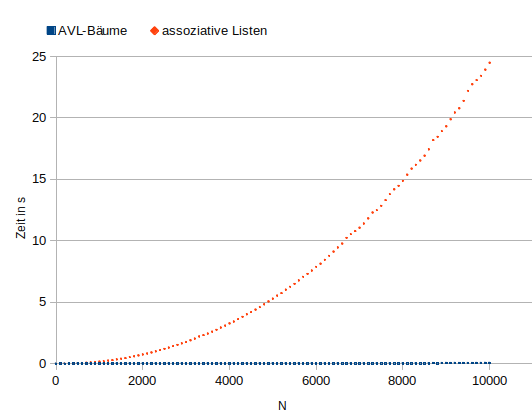
\includegraphics{bench}
  \caption{Vergleich der Einfügeoperationen von assoziativen Listen und AVL-Bäumen}
  \label{fig:avl-vs-assoc}
\end{figure}
Mithilfe des extrahierten OCaml-Codes kann nun die Laufzeit der Einfügeoperationen zwischen AVL-Bäumen und assoziativen Listen verglichen werden.
Der Vergleich ist in \autoref{fig:avl-vs-assoc} abgebildet.
Dazu wird die Zeit gemessen, die für das Einfügen von $N$ zufällig generierten Einträgen in einen leeren Baum bzw. eine leere Liste benötigt wird.
Wie der dargestellte Graph zeigt, besitzt die Einfügeoperation bei AVL-Bäumen eine wesentlich geringere Laufzeit als bei den assoziativen Listen.
Das entspricht den Erwartungen, denn für das Einfügen von einem einzelnen Element steigt bei AVL-Bäumen die Worst-Case Laufzeit nur logarithmisch mit der Anzahl der vorhandenen Elemente, während bei assoziativen Listen die Laufzeit für diese Operation linear ansteigt.
Insgesamt bedeutet das, dass die Laufzeit für das Einfügen von $N$ Elementen bei AVL-Bäumen $\mathcal{O}(N\log{}N)$ beträgt, während sie bei den assoziativen Listen $\mathcal{O}(N^2)$ beträgt, wie im Graph zu erkennen ist.
Der vollständige Quellcode für diesen Benchmark und die Implementierung der Mapping-Datenbank kann unter \autocite{source} abgerufen werden.

\begin{listing}[htp]
  \begin{minted}[fontsize=\small]{coq}
    Require MappingDB_avl.
    Require MappingDB.
    Require ExtrOcamlBasic.
    Require ExtrOcamlZInt.
     
    Require Import NArith.
     
    (* This is the only dependency remaining on N. 
     * Inlining gets rid of the dependency. 
     *
     * Note that we need to supply a definition of N.compare using 
     * parentheses here, since coq is not smart enough to automatically 
     * insert parenthesis when inlining, which produces invalid ocaml code.
     *)
    Extract Constant N.compare
      =>"(fun x y -> if x=y then Eq else if x<y then Lt else Gt)".

    (* Blacklist the List name, since OCaml uses the same name for it's 
     * list module.  
     *)
    Extraction Blacklist List. 
    (* Change to the extraction directory, so the generated files 
     * do not clutter the source directory 
     *)
     
    (* Extract AVL implementation and assoc list implementation.
     * 
     * Separate makes sure that everything gets extracted to different files, 
     * which results in much cleaner code and allows to get rid of all 
     * the NArith bloat  (the extracted NArith file can be ignored, since it
     * is not used by anything).
     *)
    Separate Extraction MappingDB_avl MappingDB AVLTree AssocList.
  \end{minted}
  \caption{Coq-Code zur Extraktion}
  \label{lst:extract}
\end{listing}

\section{Ergebnisse und Ausblick}

Während der Verifikation wurden mehrere Fehler in der Implementierung gefunden, die behoben werden mussten:
\begin{enumerate}
\item Wenn ein Knoten entfernt werden soll, der zwei nicht-leere Teilbäume hat, so muss dieser durch einen anderen Knoten ersetzt werden, an welchem die Teilbäume aufgehängt werden.
Dazu sollte normalerweise der am weitesten links stehende Knoten des rechten Teilbaums genommen werden, denn alle restlichen Knoten im rechten Teilbaum sind größer als dieser und somit wird die Invariante des binären Baums erhalten. 
In der ersten Implementierung wurde jedoch stattdessen der am weitesten rechts stehende Knoten gesucht, sodass die Invariante verletzt wurde. Dieser Fehler hätte zum Datenverlust führen können.
\item Die \verb|node|-Funktion hat eine falsche Höhenänderung zurückgegeben, falls eine doppelte Linksrotation durchgeführt werden musste. Der Fehler entstand beim Übertragen der Rechtsrotation, wobei eine Spiegelung vergessen wurde.
\end{enumerate}
Es wurden einfache Tests implementiert, um Fehler möglichst vor der Verifikation zu finden.
Damit soll verhindert werden, dass viel Zeit in einen unmöglichen Beweis investiert wird.
Diese Tests wurden allerdings manuell geschrieben und haben nur kleinere Bäume getestet, sodass diese Fehler unbemerkt blieben.
Die formale Verifikation garantiert jedoch, dass keine weiteren Fehler wie diese existieren.
Die meiste Zeit der Umsetzung wurde für die Beweise zur Erhaltung der Invarianten benötigt.
Dabei war der Beweis der AVL-Invariante weitaus aufwändiger als der Beweis der Invariante des binären Baums.

Durch die Verwendung der AVL-Bäume wird also eine effiziente Implementierung der Mapping-Datenbank erreicht. 
Die Beweise in Coq stellen sicher, dass die Implementierung auch korrekt funktioniert.
Zur Ausführung auf dem Microkern wird die Mapping-Datenbank jedoch in C implementiert.
In einem weiteren Schritt muss daher ein Refinement auf die Implementierung in C durchgeführt werden, womit gezeigt wird, dass sich die C-Implementierung genauso wie die Coq-Implementierung verhält.
Um dieses Ziel zu erreichen werden jedoch noch mehrere Zwischenschritte notwendig sein.

\newpage
\raggedright
\printbibliography[heading=bibnumbered]

\newpage

\section{Anhang}
\mbox{}
\begin{code}
  \caption{Theoreme für die Operationen der Mapping-Datenbank}
  \label{lst:db-theorems}

  \begin{minted}[fontsize=\small]{coq}
  Definition has_mapping (pd:N) (sel:N) (ko:kernel_object) : mapping_db -> Prop :=
    contains pd (In (sel,ko)).

  Definition in_mapping_db (pd:N) (sel:N) : mapping_db -> Prop :=
    contains pd (in_domain sel).

  Definition mapping_db_inv (db:mapping_db) : Prop :=
    avl_tree_invariant db /\ (forall k v, In (k,v) db -> avl_tree_invariant v).

  Theorem create_has_mapping :
    forall (db:mapping_db) (pd:N) (sel:N) (ko:kernel_object),
      mapping_db_inv db ->
      has_mapping pd sel ko (create_mapping pd sel ko db).

  Theorem create_preserve_other :
    forall (db:mapping_db) (pd pd':N) (sel sel':N) (ko ko':kernel_object),
      (pd' <> pd \/ sel' <> sel) -> mapping_db_inv db ->
      (has_mapping pd sel ko db
       <-> has_mapping pd sel ko (create_mapping pd' sel' ko' db)).

  Theorem create_invariant :
    forall (db:mapping_db) (pd:N) (sel:N) (ko:kernel_object),
      mapping_db_inv db ->
      mapping_db_inv (create_mapping pd sel ko db).

  Theorem delete_deletes_mapping :
    forall (db:mapping_db) (pd:N) (sel:N) (ko:kernel_object),
      mapping_db_inv db -> ~has_mapping pd sel ko (delete_mapping pd sel db).
  
  Theorem delete_preserve_other :
    forall (db:mapping_db) (pd pd':N) (sel sel':N) (ko:kernel_object),
      mapping_db_inv db -> (pd' <> pd \/ sel <> sel') ->
      (has_mapping pd sel ko db <-> has_mapping pd sel ko (delete_mapping pd' sel' db)).

  Theorem delete_invariant :
    forall (db:mapping_db) (pd sel:N),
      mapping_db_inv db -> mapping_db_inv (delete_mapping pd sel db).

  Theorem delete_all_except_deletes :
    forall (db:mapping_db) (pd:N) (sel:N) (ko:kernel_object) (f:kernel_object -> bool)
           (exceptions:avl_tree (list N)),
      mapping_db_inv db ->
      has_mapping pd sel ko (delete_all_except f exceptions db) ->
      f ko = false \/ contains pd (List.In sel) exceptions.

  Theorem delete_all_except_preseve_other :
    forall (db:mapping_db) (pd:N) (sel:N) (ko:kernel_object) (f:kernel_object -> bool)
           (exceptions:avl_tree (list N)),
      mapping_db_inv db ->
      f ko = false ->
      (has_mapping pd sel ko db <->
       has_mapping pd sel ko (delete_all_except f exceptions db)).

  Theorem delete_all_invariant :
    forall (db:mapping_db) (pd:N) (sel:N) (ko:kernel_object) (f:kernel_object -> bool)
           (exceptions:avl_tree (list N)),
      mapping_db_inv db -> mapping_db_inv (delete_all_except f exceptions db).
  \end{minted}
\end{code}

\begin{code}
  \caption{Definition und Invarianten des AVL-Baums}
  \label{lst:avl-def}

  \begin{minted}[fontsize=\small]{coq}
  Inductive avl_tree (T:Type) : Type :=
    (** A branch consists of a balance, the left subtree, the key + value 
     * and the right subtree. The balance is [positive] if the left subtree's
     * height is greater than the height of the right subtree. If the heights 
     * are the same, the balance is [zero], otherwise it will be [negative].
     *)
    | Avl_branch : sign -> avl_tree T -> N * T -> avl_tree T -> avl_tree T
    | Avl_empty  : avl_tree T.

  Section Invariants.

  Variable T : Type.

  Fixpoint avl_height (t:avl_tree T) : N :=
    match t with
      | Avl_empty => 0
      | Avl_branch _ l _ r => N.succ (N.max (avl_height l) (avl_height r))
    end.

  Definition balanced_with (b:sign) (l r:avl_tree T) : Prop :=
    match b with
      | positive => avl_height l = N.succ (avl_height r)
      | zero     => avl_height l = avl_height r
      | negative => N.succ (avl_height l) = avl_height r
    end.
  
  Fixpoint balance_correct (t:avl_tree T) : Prop :=
    match t with
      | Avl_empty => True
      | Avl_branch b l _ r => 
          balanced_with b l r /\ balance_correct l /\ balance_correct r
    end.

  Fixpoint forall_keys (f:N -> Prop) (t:avl_tree T) : Prop :=
    match t with
      | Avl_empty => True
      | Avl_branch _ l p r => f (fst p) /\ forall_keys f l /\ forall_keys f r
    end.


  Fixpoint binary_tree_invariant (t:avl_tree T) : Prop :=
    match t with
      | Avl_empty => True
      | Avl_branch _ l p r =>
        forall_keys (N.gt (fst p)) l /\ forall_keys (N.lt (fst p)) r /\
        binary_tree_invariant l /\ binary_tree_invariant r
    end.

    End Invariants.
  \end{minted}
\end{code}

\end{document}
%  LocalWords:  Betriebssystemkerne
